\section{Skriptiranje}
Skriptiranje (\emph{eng. scripting}) je jedan od osnovnih dijelova svaki igre jer svaku igru je potrebno definirati određena pravila, te nekakav mehanizam koji će motriti sve igrajuće objekte i provjeravati da li se drže tih pravila. Skripte isto tako omogućavaju stvaranje grafičkih efekata korištenjem ugrađenih metoda ili mijenjanje same fizike igre tokom igranja.
\subsection{Izrada i korištenje skripti}
Izrada skripti se može na više načina. Najjednostvniji način je preko botuna za dodavanje komponenti igrajućem objektu, te odabirom nova skripta (\emph{eng. new script}). Na ovaj način istovremeno se napravi skripta i pridruži igrajućem objektu. Kako je već navedno unity dopušta pisanje skripti u dva jezika:
\begin{itemize} 
	\item C\# - industrijski standard, jezik koji je veoma sličan Javi ili C++
	\item Unityscript - jezik baziran na Javascriptu
\end{itemize}
\subsection{Sadržaj skripti}
Otvaranjem novoizrađene skripte može se vidjeti sadržaj. Unity omogućava da programer sam odabere program za otvaranje skripti, ali zadani program je MonoDevelop. U ispisu \ref{primjerSkripte}  je primjer C\# skripte.

\begin{lstlisting}[caption={Primjer skripte}, label=primjerSkripte]
using UnityEngine;
using System.Collections;

public class MainPlayer : MonoBehaviour {

    void Start () {
    
    }
    
    void Update () {
    
    }
}
\end{lstlisting}
Start metoda se koristi za incijalizaciju varijabli prilikom pokretanja programa. Ova metoda \textbf{nije konstruktor}, već unity preuzima odgovornost za sve konstruktore. Velika greška bi bila definiranje specijalnih konstruktora i vrlo vjerojatno ne bi ništa radilo. \par
Druga metoda koja je generirana se pokreće za broj slika u sekundi (\emph{eng. frame per second fps}). Zanimljivo je da postoje tri varijacije ove metode.
\begin{itemize} 
	\item Update
	\item FixedUpdate - koji bi se trebao koristiti, ukoliko igrajući objekt sadrži kruto tijelo
	\item LateUpdate - se pokreće nakon svih drugih update funkcija, a korisna je za mijenjanje pozicije kamere jer se trebaju prvo pomaknuti svi objekti, a tek onda kamera. 
\end{itemize}
Kod sve tri metode se često upotrebljava varijabla \textit{Time.deltaTime}, koja je decimalna vrijednost vremena između svake slike. Ukoliko bi se željelo isprogramirati da se nešto kreće dvadeset metara po sekundi, tada se ova varijabla samo pomnoži sa brojem 20.
\subsection{Pokretanje igrajućih objekata}
Ako se napravi skripta preko \emph{Assets > Create > C\# Script}, tada prilikom pokretanja igra se skripta neće izvršavati jer nije pridružena igrajućem objektu. Samo skripte koje su pridružene igrajućim objektima će se pokretati. Za provjeru da li funkcionira skripta se može koristiti naredba za debugiranje \emph{Debug.Log("Skripta radi!")}. Kako je navedeno igrajući objekti su samo kontenjeri za komponente, što znači da ukoliko je želja upravljati igrajućim objektima potrebno je upravljati komponentama. Primjer dohvaćanja komponenti se može vidjeti u ispisu \ref{dohvacanjeObjekata}. 
\begin{lstlisting}[caption={Dohvaćanje objekata}, label=dohvacanjeObjekata]
for (int i = 0; i < 4; i++) {
	this.tires[i] = GameObject.Find(this.tireNames[i]);
	this.tirePivots[i] = GameObject.Find(this.tirePivotNames[i]);
}
\end{lstlisting}
\subsection{Funkcije događaja}
Skripte u unity-u nisu kao u drugim programskim jezicima da se vrte u beskonačnoj petlji dok ne završe dani zadatak. Unity funkcionira tako da prebacuje kontrolu funkcijama koje se trebaju izvršiti, koje nakon izvršavanja vrate kontrolu natrag unity-u. Ovakve funkcije se zovu funkcije događaja (\emph{eng. Event functions}). Neke od najučestalijih koje se koriste su:
\begin{itemize} 
	\item Regularna ažuriranja događaja (\emph{eng. Regular update events}) - sve funkcije koje se pokreću za animiranje ili manipuliranje likovima (Update, LateUpdate, FixedUpdate)
	\item Inicijalizacijski događaji (\emph{eng. Initialization Events}) - funkcije koje se pokreću na početku pokretanja unity-a. Spomenuta je Start, ali postoji i buđenje (\emph{Awake}). Awake se poziva za svaki igrajući objekt prije nego što se scena napravi. (Awake se pokreće prije Start)
	\item Fizički događaji (\emph{eng. Physics Events}) - sve funkcije koje se pokreću kada se dogodi kolizija igrajućih objekata
\end{itemize}
\begin{figure}[h]
	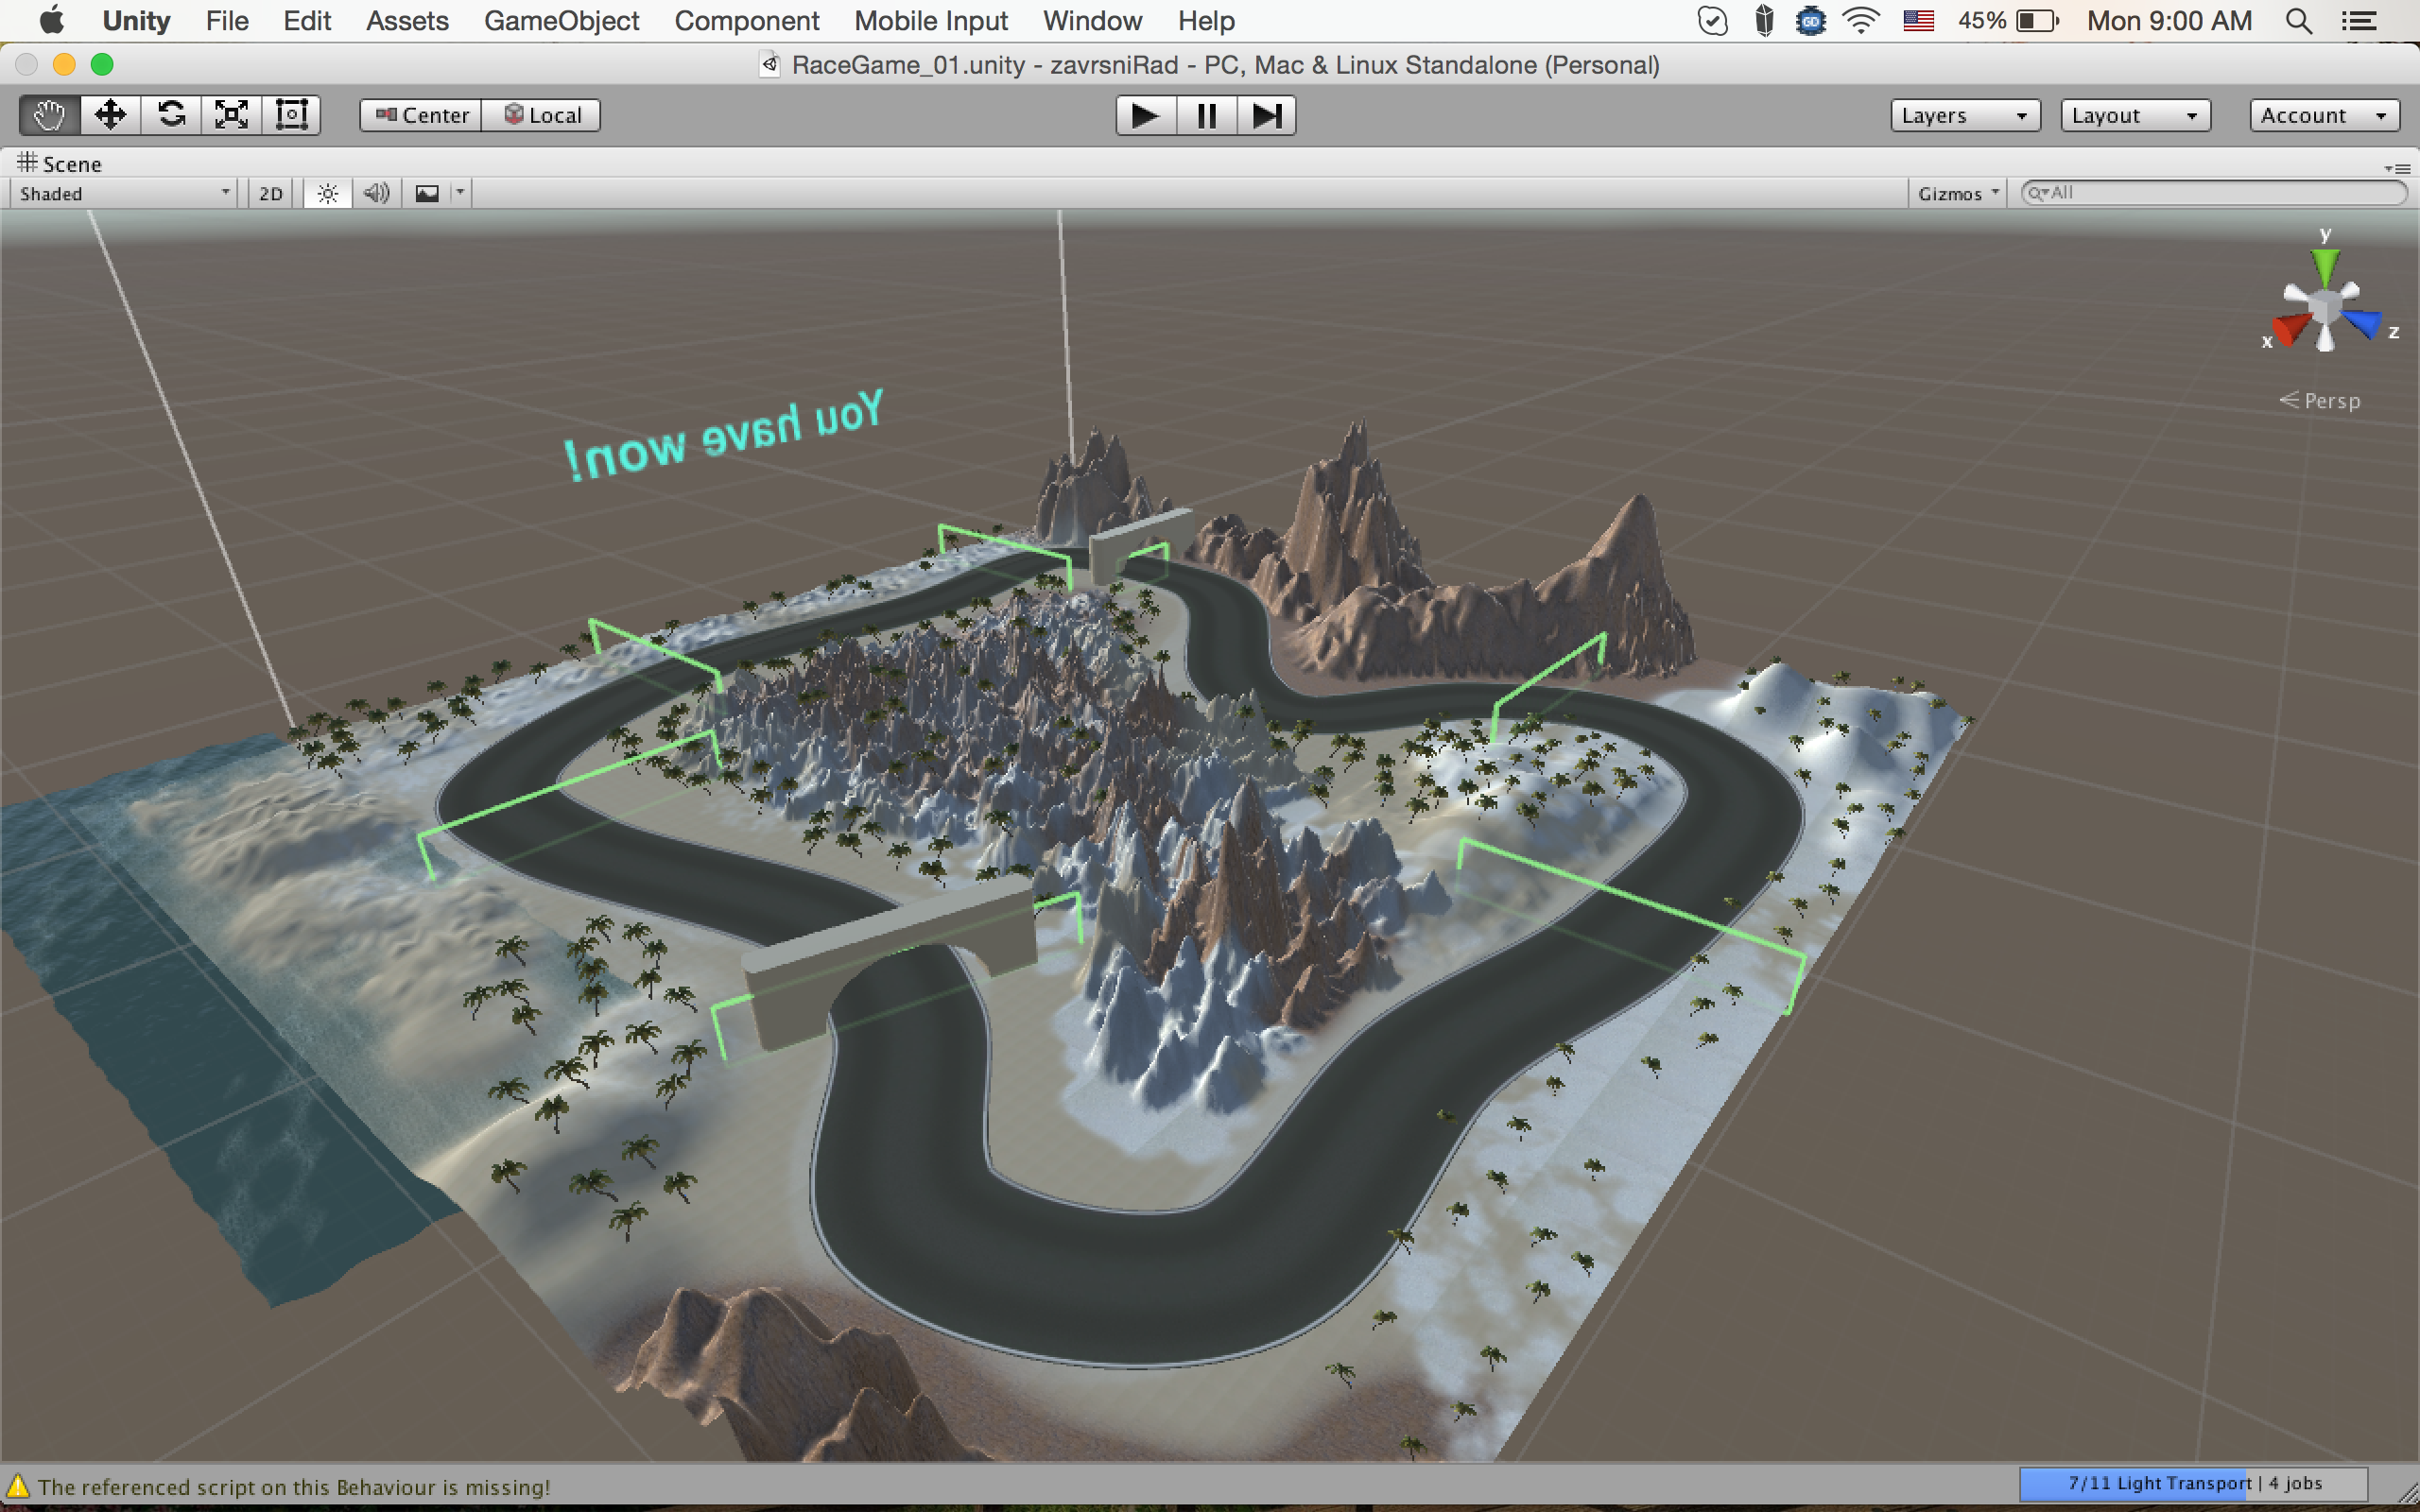
\includegraphics[width=12.5cm, height=8cm]{roadMarkers.png}
	\centering
	\caption{Markeri putanje}
	\label{fig:markeriPutanje}
\end{figure}
\subsubsection{Razlike fizičkih funkcija događaja}
Unity razlikuje dva različita tipa ovih funkcija. One koje se pozivaju prilikom kontakta sa igrajućim objektom i one koje imaju na sudaračima označeno da je okidač (\emph{eng. Trigger}). Svaka od ovih prima parametar, a isto tako se razlikuju i po tome. Imena funkcija moraju biti točno napisana i njihovi potpisi moraju biti točni, inače se neće pozivat i unity će izbaciti pogrešku. \par
Kolizijske funkcije (OnCollisionEnter, OnCollisionStay, OnCollisionExit) imaju potpis koji izgleda kao ispis \ref{potpisKolizije}. Ove metode se pozivaju kada se dva tijela koji imaju kruto tijelo ili sudarač, a sadrže informaciju o mjestu kontakta i brzini sudara.
\begin{lstlisting}[caption={Potpis kolizijskih funkcija}, label=potpisKolizije]
void OnCollisionEnter(Collision col);
\end{lstlisting} \par
Funkcije koje se pokreću na okidač (OnTriggerEnter, OnTriggerStay, OnTriggerExit) imaju kao ulazni parametar sudarač, pa je moguće više informacija saznati iz njega. Isto tako se pozivaju kada se dva tijela sudare, ako barem jedno tijelo ima svoj sudarač označen kao okidač. Potpis ove funkcije i primjer kako izgleda u igri se može vidjeti u ispisu \ref{primjerTrigger}
\begin{lstlisting}[caption={Potpis i primjer trigger funkcije}, label=primjerTrigger]
void OnTriggerEnter(Collider col) {
	if (col.gameObject.layer == LayerMask.NameToLayer ("RoadMarkers"))
		this.checkTheRightMarker (col.ToString ().Split (' ') [0]);
}
\end{lstlisting} \par
Na slici \ref{fig:markeriPutanje} se mogu vidjeti posebni markeri koji su korišteni za provjeravanje da li je automobil prešao sve markere i je li išao pravim smjerom. Ovo su obični igrajući objekti sa sudaračima kojima je označeno da su okidači. Ako se sudaraču postavi da je okidač, onda će se kroz njega moći prolaziti. 
\subsection{Generičke funkcije}
Zbog jednostavnijeg načina dohvaćanja pojedinih komponenti igrajućih objekata postoje generičke funkcije. To su funkcije koje nije potrebno eksplicitno baciti u drugi tip, već prilikom dohvaćanja definiramo tip. Primjer se može vidjeti u ispisu \ref{generickeFunkcije}
\begin{lstlisting}[caption={Primjer generičke funkcije}, label=generickeFunkcije]
this.carBody = GetComponent<RigidBody>();
\end{lstlisting}